% Sistema neumático: volumen (capacitancia C) con restricción R de entrada
\documentclass[border=5pt]{standalone}
\usepackage{tikz}
\usetikzlibrary{arrows.meta}
\begin{document}
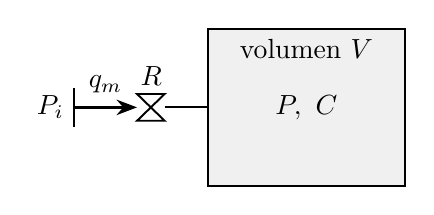
\begin{tikzpicture}[>={Stealth[length=2.6mm]}, line width=0.7pt]
  % suministro
  \node[left] at (-0.2,1.0) {$P_i$};
  \draw (-0.2,0.75) -- (-0.2,1.25);
  \draw[->, line width=1pt] (-0.2,1.0) -- (0.6,1.0);
  \node[above] at (0.2,1.05) {$q_m$};
  % restriccion R (valvula moño)
  \draw (0.6,0.83) -- (0.95,1.17) -- (0.6,1.17) -- (0.95,0.83) -- cycle;
  \node[above] at (0.78,1.15) {$R$};
  \draw (0.95,1.0) -- (1.5,1.0);
  % volumen (camara)
  \draw[fill=black!6] (1.5,0) rectangle (4.0,2.0);
  \node at (2.75,1.0) {$P,\ C$};
  \node[below] at (2.75,2.0) {volumen $V$};
\end{tikzpicture}
\end{document}
